\section{The Constrained Topographical Global Optimization Algorithm}\label{sec:Methods}

The TGO algorithm, which stands for \textit{Topographical Global Optimization}, is a meta-heuristic developed by \cite{ITGO1} for solving continuous optimization problems, possibly non-smooth and multimodal. The method has three steps: (i) the random uniform generation of a population of solutions over the domain of the problem; (ii) the selection of some of the individuals of the population based on the topography of the function to be optimized; and (iii) the application of some sort of local search in the selected elements.

Initially, the TGO creates a population of size $M$ denoted by $P = \{\bm{x}_1, \bm{x}_2, ..., \allowbreak \bm{x}_M\}$, uniformly distributed in the solution space. The TGO performance depends directly on the algorithm used in the generation of the population, and, consequently, on the pseudo-random number generator. In this work, we used the Sobol sequences \citep{Sobol, ITGO3}, which has a significantly more uniform distribution than a state-of-the-art pseudorandom number generator. Figure \ref{fig:Sobol} shows the distribution of 300 points in the domain $[0, 1]^2$, with 150 of them (blue dots) generated by the pseudo-random generator Mersenne Twister proposed by \cite{mt19937}. The other points (red dots) are the 150 first elements of a Sobol sequence. From Figure \ref{fig:Sobol} it is possible to observe that the points generated by the Sobol sequence cover the space more uniformly than those of Mersenne Twister.


\begin{figure*}[h]
\begin{center}
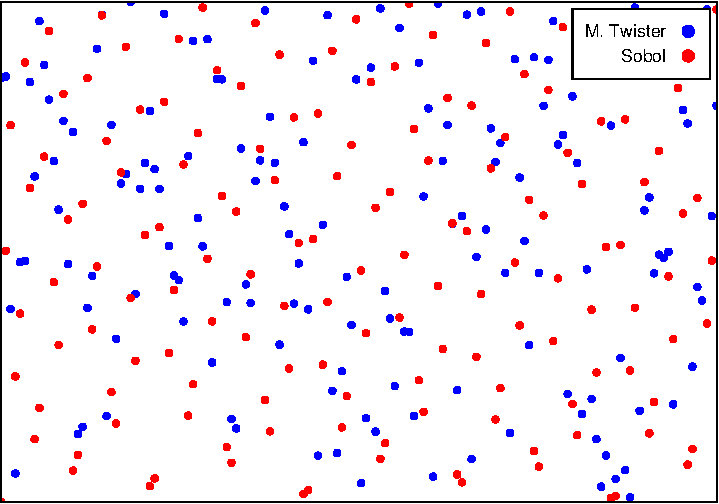
\includegraphics[scale=0.8]{scatter-crop.pdf}
\end{center}
\captionsetup{justification=centering}
\caption{Example showing the distribution of points in the domain $[0, 1]^2$ by the Mersenne Twister generator (blue points) and by a Sobol sequence (red points). }\label{fig:Sobol}
\end{figure*}


The next step is the construction of a graph over possible solutions that incorporate information regarding the topography of the function $f(\cdot)$. Consider now a integer $K > 0$. We define the $KNN_K(\bm{x})$ neighborhood as the set of the $K$ elements of the population $P$, different of $\bm{x}$, that have the smallest euclidean distance from $\bm{x}$.

A directed graph is then defined, having a vertex for every solution in the population. For each individual $\bm{x}$, a directed edge is created pointing to every element $\bm{x'}$ of the population $P$ such that $\bm{x'} \in KNN_K(\bm{x})$ and $f(\bm{x}) \leq f(\bm{x'})$. With this construction, every vertex has at most $K$ outgoing edges. A topography matrix $A \in \mathbb{R}^{M \times M}$ is created based on this graph, defined as:


\[
    A_{i, j} = 
\begin{cases}
    1,& \text{if } f(\bm{x}_i) \leq f(\bm{x}_j) \ \text{ and } \ \bm{x}_j \in KNN_K(\bm{x}_i) \\
    0,& \text{otherwise}
\end{cases}
\]
\\[-1.5em]


The matrix $A$ tells us if the element $\bm{x}_i$ has better fitness than the element $\bm{x}_j$, given that $\bm{x}_j$ is in the $KNN$ set of $\bm{x}_i$. The graph defined previously has a direct link with the topography matrix: a directed edge between elements $\bm{x}_i$ and $\bm{x}_j$ only exists if $A_{i, j} = 1$. We have then created an ordering of the elements of the population based on the position in space, the objective function value, and the neighborhood defined by $K$.

The topographic heuristic is based on selecting every individual $\bm{x}_i$ such that \allowbreak $\sum_j^M A_{i, j} = K$, that is, every individual that has better fitness than every element of its $KNN$ set. Likewise, every vertex that has $K$ outgoing edges. These elements are considered local optimal points based on the estimated topography of the function $f(\cdot)$.

As there is no guarantee that the individuals selected are really local optimal points (as we only have an estimate of the function's surface given by the topography created), the application of some algorithm for fine-tuning is necessary.

The last step of the TGO method consists in applying some sort of local search in every local optimal point based on the topographic heuristic. Regarding the local search, many procedures used in the TGO are found in the literature, such as pattern search algorithms \citep{ITGO2}, derivative-based \citep{ITGO3} and derivative-free \citep{ITGO4} optimization methods. The local search algorithm depends directly on the properties of the function to be optimized and is of significative impact in the overall performance of the method.

We consider now a simple example. Let the function $f(\cdot)$ be defined by $f(x, y) = sin(x^2) + sin(y^2)$, in the domain $[-1, 3]^2$, the population $P$ composed by the 10 elements: \\[-3em]

\begin{equation*}
  \begin{aligned}
& \qquad \bm{x}_1 = (-0.2, 0.16), \qquad \bm{x}_2 = (1.2, -0.3), \qquad \bm{x}_3 = (-0.6, 1.2) \\
& \qquad \bm{x}_4 = (-0.9, 2.4), \qquad \ \, \bm{x}_5 = (2.0, 2.0), \qquad \ \ \ \bm{x}_6 = (2.7, 0.3) \\
& \bm{x}_7 = (0.3, 2.2), \quad \bm{x}_8 = (2.0, -0.2), \quad \bm{x}_9 = (1.3, 2.8), \quad \bm{x}_{10} = (1.3, 1.2) \\
  \end{aligned}
\end{equation*}

\noindent
and the $KNN$ set determined by the $K = 3$ closest neighbors. Figure \ref{fig:Graph} shows the contour plot of the function and the directed graph created by the population. The topography matrix and the sum of each row are the following:


\[
A=
  \left(\begin{array}{cccccccccc?c}
    0 & 1 & 1 & 0 & 0 & 0 & 0 & 0 & 0 & 1 & \ \bm{3} \\
    0 & 0 & 0 & 0 & 0 & 0 & 0 & 0 & 0 & 1 & \ \bm{1} \\
    0 & 0 & 0 & 0 & 0 & 0 & 0 & 0 & 0 & 0 & \ \bm{0} \\
    0 & 0 & 1 & 0 & 0 & 0 & 0 & 0 & 1 & 0 & \ \bm{2} \\
    0 & 0 & 0 & 0 & 0 & 0 & 1 & 0 & 1 & 1 & \ \bm{3} \\
    0 & 1 & 0 & 0 & 0 & 0 & 0 & 0 & 0 & 1 & \ \bm{2} \\
    0 & 0 & 0 & 0 & 0 & 0 & 0 & 0 & 1 & 1 & \ \bm{2} \\
    0 & 1 & 0 & 0 & 0 & 1 & 0 & 0 & 0 & 1 & \ \bm{3} \\
    0 & 0 & 0 & 0 & 0 & 0 & 0 & 0 & 0 & 1 & \ \bm{1} \\
    0 & 0 & 0 & 0 & 0 & 0 & 0 & 0 & 0 & 0 & \ \bm{0} \\
  \end{array} \right)
\]
\\[-0.5em]

According with the graph and the topography matrix created, it is easy to observe that only the elements $\bm{x}_1$, $\bm{x}_5$ and $\bm{x}_8$ are local optimum, that is, has $K$ outgoing edges, satisfying $\sum_j^M A_{1, j} = \sum_j^M A_{5, j} = \sum_j^M A_{8, j} = K = 3$.

Even after the application of local search, there is no guarantee that the global optimum was found. It is common to successively apply the TGO method many times, with new elements at each iteration. This procedure is called \textit{ITGO} (\textit{Iterative Topographical Global Optimization}), and consists simply in the iterative application of the TGO method, returning the best element found during all the process.



\begin{figure*}[tp]
\begin{center}
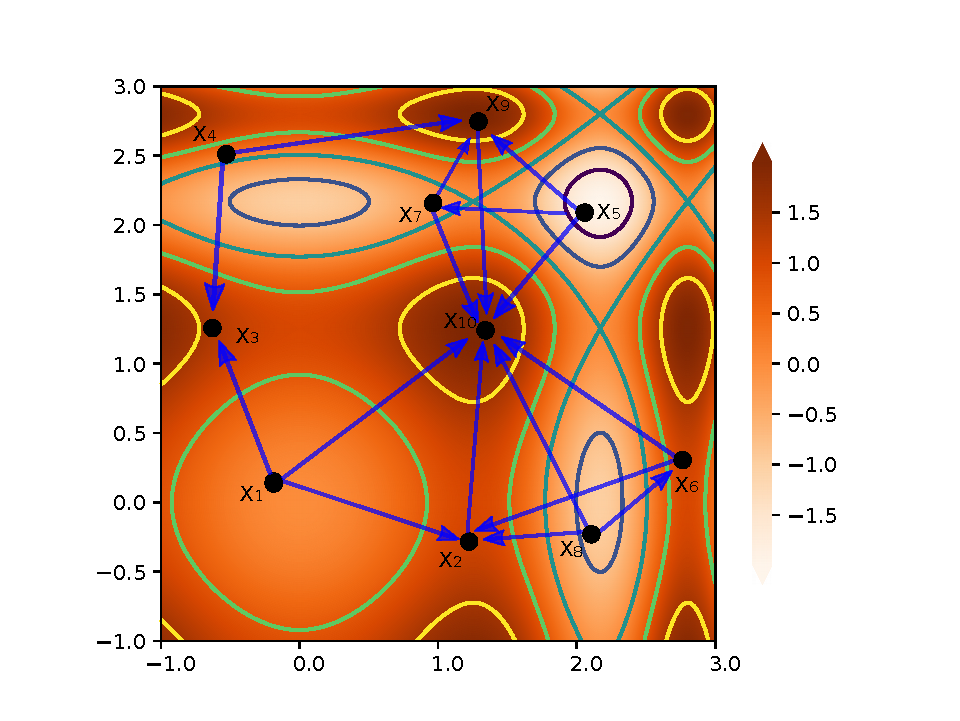
\includegraphics[scale=0.6]{fig_1_t.pdf}
\end{center}
\captionsetup{justification=centering}
\vspace*{-7mm} 
\caption{Contour plot of the function $f(x, y) = sin(x^2) + sin(y^2)$, and the graph based on the population.}\label{fig:Graph}
\end{figure*}


\subsection{Space Reduction}

In \cite{ITGO4} a heuristic for space reduction is proposed for the ITGO. After the individual selection step, a sub-space is created around every element, with space reduced in each dimension by $\phi \in (0, 1)$. A new population is generated for every space created, and new elements are selected, for each population. The process is repeated for a defined number of iterations until the execution of local search on selected elements of the last space reduction.

An example involving the application of this heuristic is presented in Figure \ref{fig:SpaceReduction}, again for the function $f(x, y) = sin(x^2) + sin(y^2)$, in the domain $[-1, 3]^2$, with the first population composed by the same 10 points described previously. Figure \ref{fig:SpaceReduction-a} shows the selection of the points $\bm{x}_1$, $\bm{x}_5$ and $\bm{x}_8$, with a space reduced by $\phi = 0.25$. Figure \ref{fig:SpaceReduction-b} we can observe the generation of populations for each new subspace. The red points are the individuals considered local optimum based on the topographic heuristic. It is worth noting that the local optimal points of the previous population are kept in the next population.


\begin{figure}[tp]
\centering
\begin{subfigure}{.5\textwidth}
  \centering
  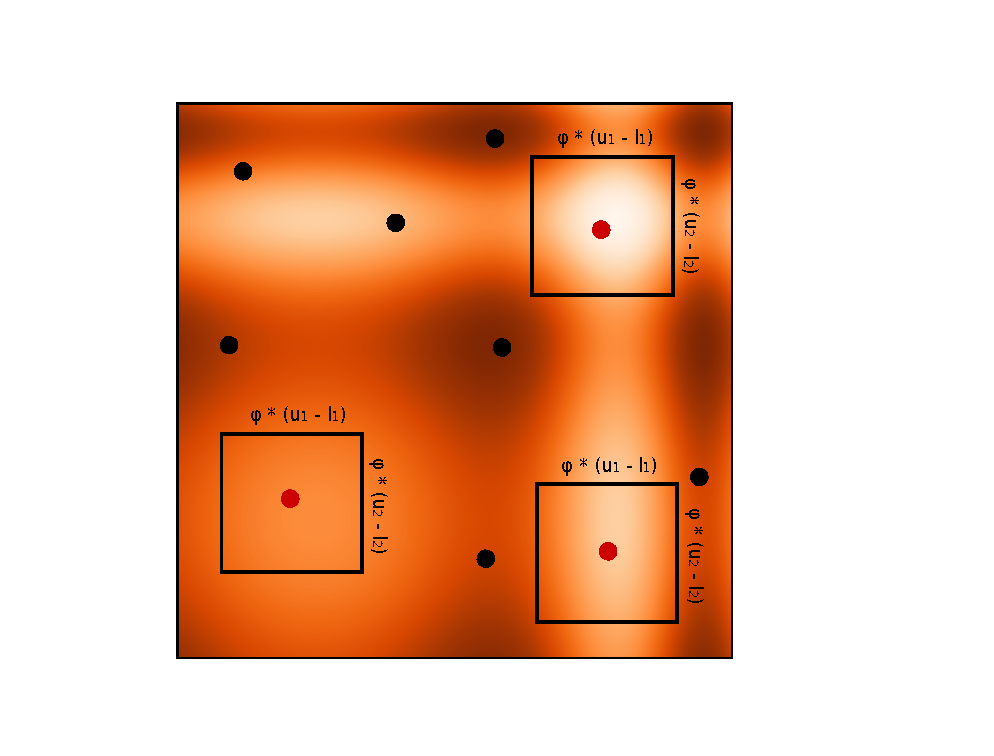
\includegraphics[width=1.1\linewidth]{fig_2.eps}
  \caption{}
  \label{fig:SpaceReduction-a}
\end{subfigure}%
\begin{subfigure}{.5\textwidth}
  \centering
  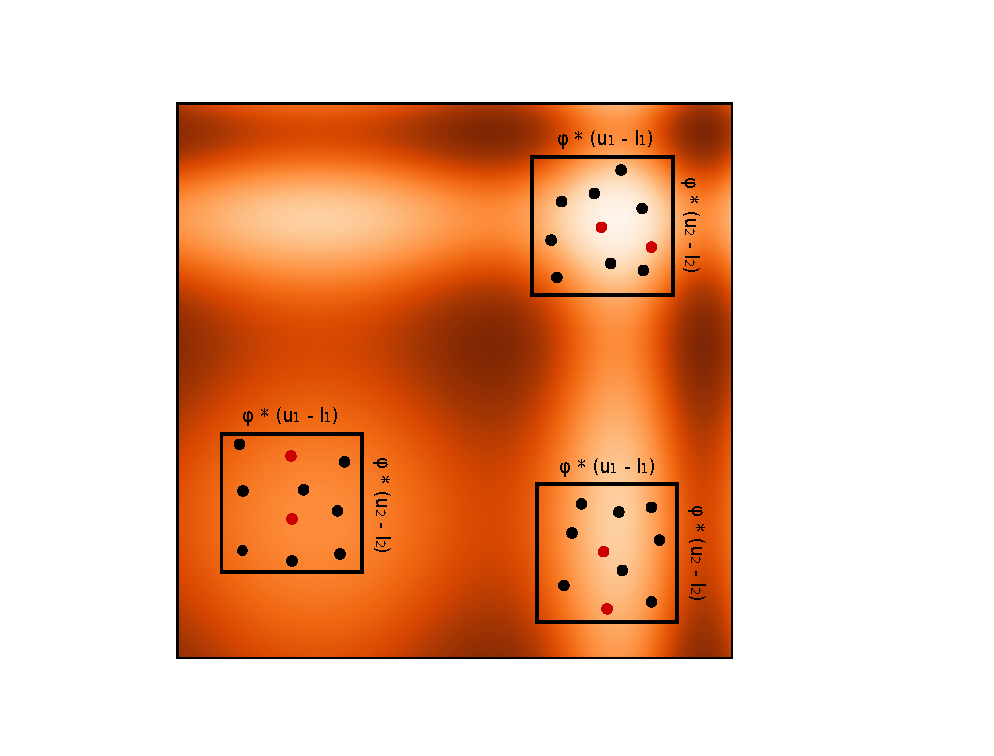
\includegraphics[width=1.1\linewidth]{fig_3.eps}
  \caption{}
  \label{fig:SpaceReduction-b}
\end{subfigure}
\caption{Example showing the application of the space reduction heuristic. In (a) we have the space reduction around the three individuals of Figure 2 ($\bm{x}_1$, $\bm{x}_5$ and $\bm{x}_8$) in red. In (b) are the respective populations generated in each restricted space to apply ITGO, with the local optimal points in red.}\label{fig:SpaceReduction}
\end{figure}


At each iteration, a new population size is set, along with a new value for $K$, which is usually smaller than in the previous iteration.


\subsection{Constrained Optimization}

Up to this point, the ITGO algorithm has been presented only for unconstrained optimization problems. ITGO was applied previously to constrained optimization problems \citep{ITGO2, ITGO3}, handling constraints by using a specific local search procedure or by penalizing unfeasible individuals.

In this work, we propose a different approach, adopting a mechanism for comparing solutions proposed in \cite{ConHandling}, and used in some very competitive meta-heuristics, especially on differential evolution algorithms \citep{DE1, DE2, DE3}. As in this work we propose a constrained version of ITGO, in the rest of the paper it is named as C-ITGO, standing for Constrained ITGO. The method for comparison used in this work hereafter comprises the following three steps criteria:

\begin{itemize}

\item Between two feasible solutions, the fittest one is better.

\item A feasible solution is always preferred over an unfeasible solution, irrespectively of its fitness.

\item Between two unfeasible solutions, the one with the smallest sum of constraint violation (equation \ref{eq:viol}) is better.

\end{itemize}


In the topographical heuristic step, we compare two solutions using this three steps criteria with probability $\alpha$, and otherwise, we compare only the fitness value. What we try to achieve with this heuristic is keeping promising solutions with small violation of constraints for further exploration with the local search step.

We generate a symmetric matrix of random numbers $R$, with $R_{i, j} = R_{j, i} \in [0, 1]$. If $R_{i, j} < \alpha$, then we compare elements $\bm{x}_i$ and $\bm{x}_j$ using the three steps criteria. Otherwise, only the fitness value is compared. In general, with this configuration, the number of local optimal points selected by the topographical heuristic is smaller, especially on problems with a small feasible area. 

It is important to observe that some distributions of the individuals, with populations of small size and a high value for $K$, may not generate any local optimum in the topographical heuristic. In the case of none of the individuals being selected as a local optimum in the current population, we take the best individual according to the three steps criteria previously presented as the only local optimum of that population. In practice, however, it is rather unusual to happen.

The best individual in the whole search is always selected using the three steps criteria already mentioned since feasible solutions are generally preferred. In addition to this new topographical selection method, we also use local search algorithms for constrained optimization.


\subsection{Implementation} \label{sec:Implementation}

We now present an overview of the implementation of the method, along with pseudocodes describing all necessary steps. Algorithm \ref{alg:ITGO} shows the general procedure for the C-ITGO algorithm.

The parameters are the functions $f(\cdot)$ and $v(\cdot)$, which return the function value and the sum of constraints violation respectively, as defined in equations \ref{eq:func} and \ref{eq:viol}, the lower and upper bound vectors $\bm{l}$ and $\bm{u}$, the vector of population sizes $\bm{PS}$, the vector of the $K$ values $\bm{KS}$, the maximum number $Max\_LS$ of elements to execute the local search, the maximum number of function calls allowed in the local search, $LS_1$ and $LS_2$, the space reduction factor $\phi$ and the probability for the three steps comparison $\alpha$.



\begin{breakablealgorithm}
\caption{CI-TGO($f(\cdot)$, $v(\cdot)$, $\bm{l}$, $\bm{u}$, $\bm{PS}$, $\bm{KS}$, $Max\_LS$, $LS_1$, $LS_2$, $\phi$, $\alpha$)}
\label{alg:ITGO}
\begin{spacing}{1.5}
\begin{algorithmic}[1]

%\State $Population \gets \{\};$
\Statex
\State $\bm{best} \gets random(\bm{l}, \bm{u});$
%\NoNumber{}


\While{$Converged(\bm{best}) == \textbf{False}$}

\State $Populations \gets \{\bm{x} = \bm{x}^1, ..., \bm{x}^{\bm{PS}(1)} : \bm{x} \in random(\bm{l}, \bm{u}) \};$
\State $TopoBest \gets \{\};$

%\NoNumber{}

\For{$p \in \{1, ..., |\bm{PS}|\}$}
%\State $ps \gets \bm{PS}(numPs);$
\State $NewPops \gets \{\};$
%\NoNumber{}

\For{$pop \in Populations$}

\State $Topo_p \gets TopographicalHeuristic(f(\cdot), v(\cdot), pop, \bm{KS}(p), \alpha);$


\If{$p < |\bm{PS}|$}

\For{$\bm{x} \in Topo_p$}
\State $NewPops \gets NewPops \ \cup \ CreatePop(\bm{x}, \bm{l}, \bm{u},\bm{PS}(p+1), \phi^p);$
\EndFor

\Else
\State $TopoBest \gets TopoBest \cup Topo_p;$
\EndIf
\EndFor

\If{$p < |\bm{PS}|$}
\State $Populations \gets NewPops;$
\EndIf
\EndFor

\State $TopoBest \gets \{\bm{x} = \bm{x}^1, ..., \bm{x}^{min(|TopoBest|, Max\_LS)} : \bm{x} \in sort(TopoBest)\};$

\For{$\bm{x} \in TopoBest$}

\State $\bm{x} \gets LocalSearch(f(\cdot), v(\cdot), \bm{x}, LS_1);$


\If{$Compare(f(\cdot), v(\cdot), \bm{x}, \bm{best})$ \ \textbf{or} \ $f(\bm{x}) < f(\bm{best})$}

\State $\bm{x} \gets LocalSearch(f(\cdot), v(\cdot), \bm{x}, LS_2);$


\If{$Compare(f(\cdot), v(\cdot), \bm{x}, \bm{best})$}
\State $\bm{best} \gets \bm{x};$
\EndIf
\EndIf

\EndFor

\EndWhile

\State \Return $best;$


\end{algorithmic}
\end{spacing}
\algcomment{Pseudocode for Constrained I-TGO.}
\end{breakablealgorithm}


The first line initializes the vector $\bm{best}$ randomly within the range $[\bm{l}, \bm{u}]$, which is the variable that saves the best element found in the search. The main loop starts at line 2, where we check for convergence. The function $Converged$ is problem dependent and may take into account the number of iterations, the number of function calls, the convergence of the best individual or any other stopping criteria.

Line 3 initializes the vector of current populations, with all the $\bm{PS}(1)$ elements inside the bounds of the problem ($[\bm{l}, \bm{u}]$). We use $random$ here to denote the generation of a random scalar or vector for simplicity, although in the implementation we used Sobol sequences for the generation of the individuals. The set $TopoBest$ at line 4 comprises the best local optimum elements found in all populations and is initialized empty.

For each population size (line 5), which is the number of space reductions plus one, we generate new populations, starting from the empty set at line 6. Here, we use $|\cdot|$ to denote the number of elements inside a set or a vector. Line 7 loops through all the populations and execute the topographical heuristic ($TopographicalHeuristic$ function), with $K = \bm{KS}(p)$. The variable $Topo_p$, at line 8, saves the local optimal points selected from the current population.

If the current space reduction is not the last ($p < |\bm{PS}|$, line 9), we create a new population around every point in the $Topo_p$ set, with size $\bm{PS}(p + 1)$ and space reduced at every dimension by $\phi^p$ (lines 10 and 11). Otherwise, if it is the last space reduction, we have to save the local optimal points in the set $TopoBest$ (lines 12 and 13) to apply local search.

The $CreatePop$ procedure is shown in algorithm \ref{alg:CreatePop}. Given an individual $\bm{x}_b$ (a selected local optimum), the function returns a new randomly generated population with $popSize-1$ individuals around this solution, in the original space reduced by the fraction $\phi$. If the point is closer than $0.5 * (u_i - l_i), \ i = 1, ..., n$, from the lower or upper bounds at dimension $i$, the limits of that new population are taken to be the original bounds. The $min$ and $max$ operations are executed element by element. The solution $\bm{x}_b$ is also added to the new population.\\[-1em]


\begin{breakablealgorithm}
\caption{CreatePop($\bm{x}$, $\bm{l}$, $\bm{u}$, $popSize$, $\phi$)}
\label{alg:CreatePop}
\begin{algorithmic}[1]

\State $\bm{l}' \gets max(\bm{l}, \bm{x} - (0.5 * \phi) * (\bm{u} - \bm{l}));$
\State $\bm{u}' \gets min(\bm{u}, \bm{x} + (0.5 * \phi) * (\bm{u} - \bm{l}));$
\State $Population \gets \{\bm{x} = \bm{x}^1, ..., \bm{x}^{popSize} : \bm{x} \in random(\bm{l}', \bm{u}')\};$

\State \Return $Population;$

\end{algorithmic}
\algcomment{Create a new population shrinked by $\phi$ around the point $\bm{x}$.}
\end{breakablealgorithm}


Going back to algorithm \ref{alg:ITGO}, at line 14, we check again if the current space reduction is not the last, and update the current populations at line 15, if the condition holds. Line 16 selects the $Max\_LS$ best elements of the set $TopoBest$, using the three steps criteria comparison as the sorting criteria. If $|TopoBest| < Max\_LS$, we keep all the elements.

We loop through all the elements of the now sorted $TopoBest$ set at line 17, and apply local search, with at maximum $LS_1$ function evaluations, at line 18. The function $Compare$ (line 19) is the three steps comparison, returning true if the first solution (third argument) is better than the second solution (fourth argument), and returns false otherwise. The element returned by the local search procedure is compared against the best element found in the whole search at line 19. If it is better than the best element found (according to the three steps criteria), or if its fitness is better, a new local search procedure is applied, now with $LS_2$ iterations, at line 20.

%The number of function calls is generally the determining factor of performance, so we wish to make the smallest number of local search iterations as possible since a call for the local search for each individual, in general, does hundreds or thousands of function evaluations.

The number of function calls is usually the determining performance factor. So, we wish to do as few local search iterations as possible, since a call to the local search algorithm typically makes hundreds or thousands of function evaluations. Here, we set $LS_2 > LS_1$, so every element undergoes $LS_1$ function evaluations in the local search, but we only search finely for promising solutions, setting higher values for $LS_2$. Usually, the second local search is only necessary for problems where very finely tuned solutions are required.

At line 21 we compare again the solution generated by the second local search ($\bm{x}$) against the best element found in the whole search ($\bm{best}$) using the three steps criteria. If the new solution is better, we set $\bm{best}$ to that solution at line 22 and continue the loop for applying local search in the other elements. At the end of the execution, when $Converged$ in the outer loop returns true, we return the best solution found in the whole search on line 23. In practice, however, we may stop the algorithm as soon as the optimal solution is found or when the maximum number of function evaluations is reached.

Finally, let us explain the $TopographicalHeuristic$ procedure, shown in Algorithm \ref{alg:TopographicalHeuristic}. The function takes as parameters: the objective function $f(\cdot)$, the sum of constraints function $v(\cdot)$, the current population to be evaluated, the value $K$ for the $KNN$ set, and the probability $\alpha$, for the three steps comparison.


\begin{breakablealgorithm}
\caption{TopographicalHeuristic($f(\cdot)$, $v(\cdot)$, $Population$, $K$, $\alpha$)}
\label{alg:TopographicalHeuristic}
\begin{spacing}{1.5}
\begin{algorithmic}[1]


\State $M \gets |Population|;$
\State $\bm{best} \gets Population(0);$
\State $KNN_K \gets Build\_KNN(Population, K);$
\State $\bm{R} \gets random([0, 1]^{M \times M});$
\State $TopoBest \gets \{\};$
%\State $\bm{Dist}_{i, j} \gets \{|Population(i) - Population(j)|, \ i, j \in \{1, ..., |Population|\}\};$ 

\For{$i \in \{1, ..., |Population|\}$}

\State $insert \gets \bm{True};$

\For{$j \in \{1, ..., |Population|\} \ \cap \ \{\bm{x}_j \in KNN_K(\bm{x}_i)\}$}
	\If{$\bm{R}_{i, j} < \alpha$}
		\State $insert \gets insert$ \& $Compare(f(\cdot), v(\cdot), \bm{x}_i, \bm{x}_j);$
	\Else
		\State $insert \gets insert$ \& ($f(\bm{x}_i) < f(\bm{x}_j));$
	\EndIf
\EndFor

\If{$insert = \bm{True}$}
\State $TopoBest \gets TopoBest \ \cup \ \{\bm{x}_i\};$
\EndIf

\If{$Compare(f(\cdot), v(\cdot), \bm{x}_i, \bm{best})$}
\State $\bm{best} \gets \bm{x}_i;$
\EndIf
\EndFor

\If{$|TopoBest| = 0$}
	\State $TopoBest \gets \{\bm{best}\};$
\EndIf

\State \Return $TopoBest;$



\end{algorithmic}
\end{spacing}
\algcomment{Topographical heuristic procedure.}
\end{breakablealgorithm}


Lines 1-5 of Algorithm \ref{alg:TopographicalHeuristic} simply initialize the necessary structures. Namely, the number of elements $M$ in $Population$, the $\bm{best}$ vector, which is the best element of the entire population based on three steps comparison (initially set to any individual of the population), the $KNN_K$ structure based on the elements of the population, which is a mapping from a solution vector $\bm{x}$ to a set of the vectors that belong to the $KNN_K$ of $\bm{x}$, the random symmetric matrix $R$, with every element in the range $[0, 1]$, and the $TopoBest$ set, containing the local optimal points, initially empty.

At line 6 we loop through all indices of $Population$, and set the $insert$ flag to $\bm{True}$ at line 7, which indicates if the individual $\bm{x}_i$ is a local optimal point. For every index $j$, such that $\bm{x}_j$ is in the set $KNN_K(\bm{x}_i)$ (line 8), we compare $\bm{x}_j$ with $\bm{x}_i$. If $R_{i, j} < \alpha$, then we set the flag $insert$ to the boolean result of the \textit{and} operator ($\&$) to $insert$ and the result of $Compare$ (lines 9-10). That is, if $Compare$ returns false at least one time for any $j$, $insert$ will also be false for the index $i$. If $R_{i, j} >= \alpha$, then we execute the same procedure, but now using fitness only comparison, at lines 11-12.

At line 13 we check if $insert = \bm{True}$, and, if so, $\bm{x}_i$ is a local optimum, and we insert it in the $TopoBest$ set, at line 14. Lines 15-16 select the best element found in the whole population based on the three steps comparison, and stores that solution in the variable $\bm{best}$. In case of no solution being selected as a local optimum, the set $TopoBest$ is composed only of the $\bm{best}$ element (lines 17-18). At line 19 we return the $TopoBest$ set, containing all the local optimal points (or the $\bm{best}$ element).


\subsection{Local Search}

In this section, we discuss the three different methods of local search we have chosen in the present work to be used in C-ITGO, and their implications on the final performance.

As we used Matlab to implement C-ITGO, a natural choice for the local search step is the use of the optimization toolbox. In the case of real non-linearly constrained problems, we used the \textit{SQP} (Sequential Quadratic Programming), present in the \textit{fmincon} package \citep{fmincon}. The basic SQP algorithm is described in Chapter 18 of \cite{Nocedal}, although the actual implementation used in fmincon uses some additional heuristics. 

A very successful method, also implemented in Matlab, that uses that same package (SQP of fmincon) is the \textit{MVMO} (Mean-Variance Mapping Optimization) \citep{MVMO}, winner of two different categories of the IEEE Congress on Evolutionary Computation competition on real optimization in 2016.

For mixed integer problems with nonlinear constraints, we used the \textit{OPTI} toolbox \citep{OPTI}, which has many algorithms specialized for mixed integer programming. Specifically, we used the \textit{BONMIN} (Basic Open-source Nonlinear Mixed INteger programming) \citep{BONMIN} and the \textit{NOMAD} (Nonlinear Optimization with the MADS algorithm) solvers \citep{NOMAD}.

We emphasize here that any kind of local search can be used in conjunction with C-ITGO. We could use for example a specialized local search for a given problem. In this work, both problems on continuous and integer domains are treated in the same way, changing only the local search procedure.

It is true that some simpler problems can be solved solely by using an exact method such as those cited above, for example by calling the procedure at different random points. However, in multimodal objective functions with nonlinear constraints, it is usually not possible to find the global optimum. Even if a problem can be solved by an exact method, the number of function evaluations may be very large.

The objective is not to rely heavily on the local search procedure. Rather, what we want to achieve with the topographical heuristic is to provide solutions that are close to a local or global optimum, so that any reasonably good local search can converge with relative ease. In this work, the maximum number of function evaluations allowed in the first call to the local search procedure is kept as small as possible, and, in most cases, it is enough to find optimal or nearly optimal solutions.



\subsection{Parameters chosen for the engineering design problems}

Given the differences in the number of variables, constraints, size of the space, number of function calls to converge reported by competing methods, and general complexity of the problems considered in this work, we selected experimentally specific parameters for each problem aiming to obtain the best performance of C-ITGO. This is a general approach taken for most of the optimization methods compared here. The parameters were selected so as to find optimal or near-optimal solutions while minimizing the number of function evaluations (NFEs).

Table \ref{tab:Parameters} shows the choice of the parameters for the eight engineering design problems we consider: Welded Beam (WB), Tension/Compression Spring (TC), Three-Bar truss (TB), Speed Reducer I and II (SRI and SRII), Pressure Vessel (PV), Gear Train (GT) and Multiple Disk clutch brake (MD). We will comment each problem and the results obtained by C-ITGO and other competing methods in Section \ref{sec:Results}.




\begin{table*}[tp]
    \tiny
\begin{center}
\begin{tabular}{ | P{0.8cm} | P{0.8cm} | P{0.8cm} | P{0.8cm} | P{0.8cm} | P{0.8cm} | P{0.8cm} | P{0.8cm} | P{0.8cm} | P{0.9cm} | P{0.9cm}  | }
\hline
$\bm{Prob / \allowbreak Param}$ & $\bm{PS_1}$ & $\bm{PS_2}$ & $\bm{K_1}$ & $\bm{K_2}$ & $\bm{\alpha}$ & $\bm{\phi}$ & $\bm{LS1}$ & $\bm{LS2}$ & $\bm{MaxLS}$ & $\bm{LSType}$ \\
\hline

\textbf{WB} & 100 & 10 & 10 & 3 & 0.5 & 0.2 & 100 & 200 & 5 & \textbf{SQP} \\
\textbf{TC} & 50 & 10 & 8 & 3 & 0.5 & 0.2 & 100 & 200 & 5 & \textbf{SQP} \\
\textbf{TB} & 30 & 5 & 5 & 2 & 0.5 & 0.2 & 20 & 70 & 5 & \textbf{SQP} \\
\textbf{SRI} & 150 & 10 & 10 & 3 & 0.5 & 0.2 & 100 & 200 & 5 & \textbf{BONMIN} \\
\textbf{SRII} & 100 & 10 & 10 & 3 & 0.5 & 0.2 & 50 & 100 & 5 & \textbf{SQP} \\
\textbf{PV} & 50 & 10 & 8 & 3 & 0.5 & 0.5 & 30 & 100 & 5 & \textbf{BONMIN} \\
\textbf{GT} & 20 & 5 & 5 & 2 & 0.5 & 0.7 & 30 & 100 & 5 & \textbf{NOMAD} \\
\textbf{MD} & 20 & 5 & 7 & 2 & 0.5 & 0.7 & 100 & 200 & 5 & \textbf{NOMAD} \\
\hline

\end{tabular}
\end{center}
\vspace*{-6mm}
\caption{Parameters of C-ITGO for each engineering design problem. \\[1em]}
\label{tab:Parameters}
\end{table*}



For all problems, we only use a single space reduction, which generates two populations and two values for $K$, namely $PS_1$ (first population size, before space reduction) and $PS_2$ (second population size, after space reduction), $K_1$ and $K_2$ (also before and after space reduction, respectively). For problems with a considerably large number of variables, it may be beneficial to use more than one space reduction.

The first population size is generally chosen to be proportional to the problem's domain size. For problems with a larger number of variables, we set $PS_1$ to 100 or above. The second population size, $PS_2$, was defined based on the first population size. For $PS_1 \geq 50$, we set $PS_2 = 10$, and for $PS_1 < 50$, $PS_2$ is set to 5.

The values of $K_1$ and $K_2$ also were chosen experimentally, but were based on the values of $PS_1$ and $PS_2$, respectively. $K_1$ was set to a maximum of 10 for larger problems, and for a minimum of 5 for small problems. For $PS_2 = 10$, $K_2$ was set to 3, and for $PS_2 = 5$, $K_2$ is 2.

The value for the probability $\alpha$ was kept constant at 0.5 for all problems. The $\alpha$ parameter controls the probability of executing the three steps comparison in the topographical heuristic step. For problems which the feasible area is small compared to the whole domain, increasing the value of $\alpha$ have the effect of reducing the number of local optimum points. However, the C-ITGO algorithm is not too sensitive to specific values of $\alpha$, and the value of 0.5 seems to be a good choice.

The maximum number of elements to execute the local search, $MaxLs$, was also set to a default value for all problems, namely 5. It acts as a filter, selecting only the best solutions to undergo the local search procedure. For problems with a large number of local optima, setting $MaxLs$ to higher values may improve C-ITGO performance. However, if $MaxLs$ is too large, many unnecessary runs of the local search will be executed.


The value of $\phi$ was set to smaller values for problems defined on entirely continuous domains and assumed higher values for mixed integer problems. If we reduce the space too much for integer problems, we may end up with some dimensions having a very small domain, possibly excluding the global optimum.

The $LS_1$ and $LS_2$ parameters control the maximum number of allowed function evaluations in the local search in the first and second calls, respectively. We tried to set $LS_1$ as small as possible while attaining convergence to the required precision (which is specific for each problem). $LS_2$ assumed higher values for more difficult problems, where convergence is achieved only for solutions very close to the global optimum.

Finally, $LSType$ represents the algorithm used in the local search. The type of local search was determined based on the properties of each problem. For problems with only continuous variables, we used the SQP method (WB, TC, and TB). For problems with only discrete variables, we used the NOMAD solver (GT, MD), and for mixed integer problems, we used the BONMIN solver (SRI and PV). The only exception was SRII, in which we used the SQP algorithm rounding the variables that are required to be integers. In tests with this specific problem (SRII), it resulted in better solutions with a smaller number of function evaluations (NFEs) than using the mixed integer solvers.